% Created 2020-05-07 Thu 18:59
% Intended LaTeX compiler: pdflatex
\documentclass[presentation]{beamer}
\usepackage[utf8]{inputenc}
\usepackage[T1]{fontenc}
\usepackage{graphicx}
\usepackage{grffile}
\usepackage{longtable}
\usepackage{wrapfig}
\usepackage{rotating}
\usepackage[normalem]{ulem}
\usepackage{amsmath}
\usepackage{textcomp}
\usepackage{amssymb}
\usepackage{capt-of}
\usepackage{hyperref}
\usetheme{UoB}
\author{Mark Blyth}
\date{}
\title{SOTA GPRs for neural data}
\hypersetup{
 pdfauthor={Mark Blyth},
 pdftitle={SOTA GPRs for neural data},
 pdfkeywords={},
 pdfsubject={},
 pdfcreator={Emacs 26.3 (Org mode 9.1.9)}, 
 pdflang={English}}
\begin{document}

\maketitle

\section{Background}
\label{sec:orgd705aaf}
\begin{frame}[label={sec:org1b2fac8}]{Goals}
\begin{itemize}
\item Redraft the continuation paper
\begin{itemize}
\item Week 1
\end{itemize}
\item Implement and test some GP schemes
\begin{itemize}
\item Week 2
\end{itemize}
\end{itemize}
\end{frame}

\section{GPs}
\label{sec:org2322b8f}
\begin{frame}[plain,label={sec:org93e06e4}]{My SEKernel}
\begin{center}
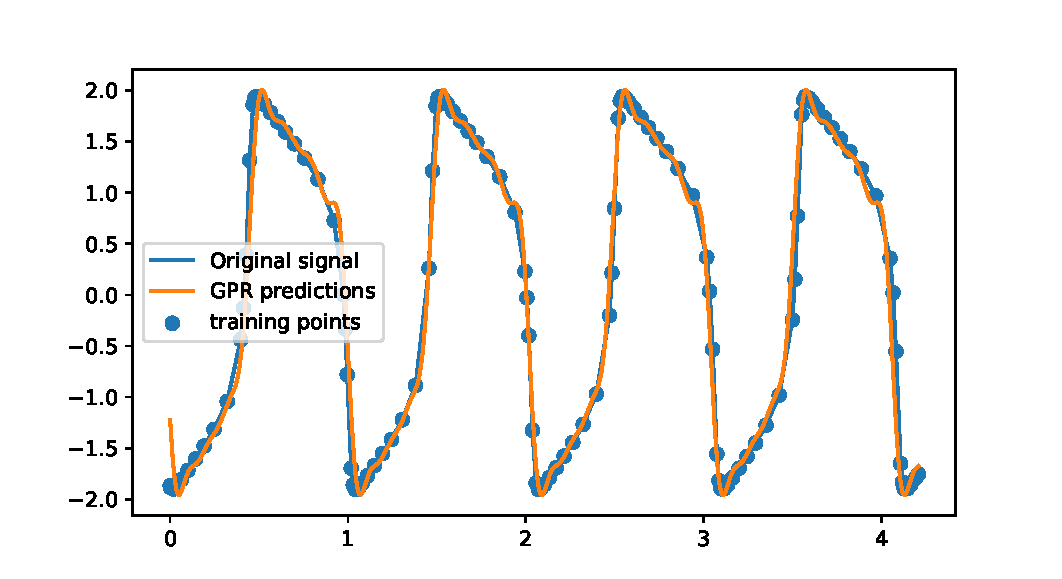
\includegraphics[width=\textwidth]{./cosinekernel1.pdf}
\end{center}

\vfill
Reasonable fit, but fixed lengthscales means it struggles at timescale changes. Good baseline. Bad for real neurons.
\end{frame}

\begin{frame}[plain,label={sec:org16b230b}]{My SEKernel}
\begin{center}
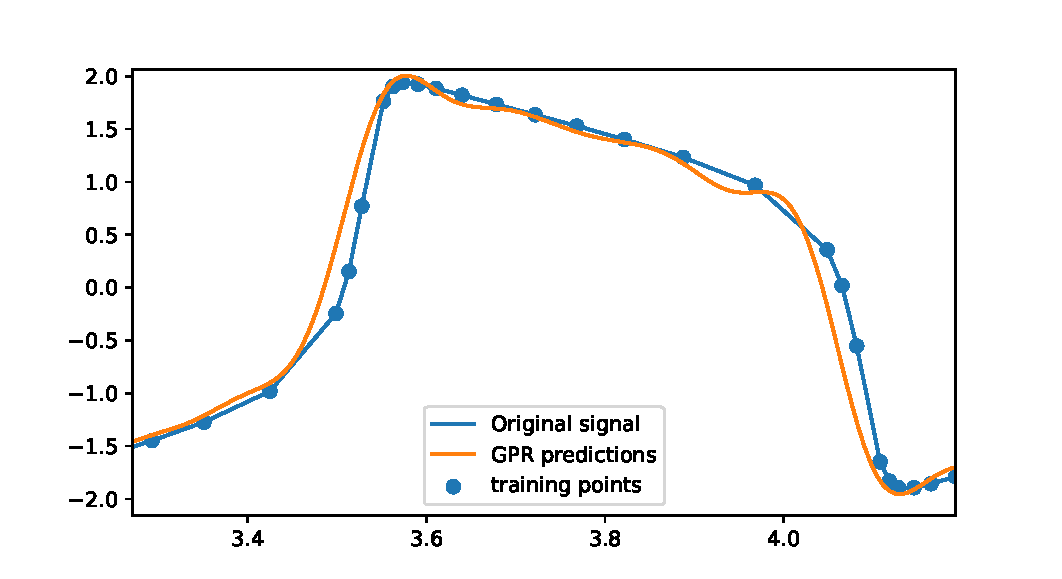
\includegraphics[width=\textwidth]{./cosinekernel2.pdf}
\end{center}

\vfill
Reasonable fit, but fixed lengthscales means it struggles at timescale changes. Good baseline. Bad for real neurons.
\end{frame}

\begin{frame}[label={sec:org68c6498}]{Generalised nonstationary spectral kernels}
\begin{itemize}
\item Method identified in the literature review as being applicable to neuron data
\item Fits into a sparse GP framework -- good for experiments
\item Models nonstationarity -- varying length scales, function variance
\begin{itemize}
\item Lengthscales quantify local similarity (think: wiggliness)
\item Multiple timescale dynamics means wiggliness changes across the signal
\end{itemize}
\item Open source code available!
\end{itemize}

\vfill
\url{https://github.com/sremes/nssm-gp}
\end{frame}

\begin{frame}[plain,label={sec:org7293dee}]{Published results}
\begin{center}
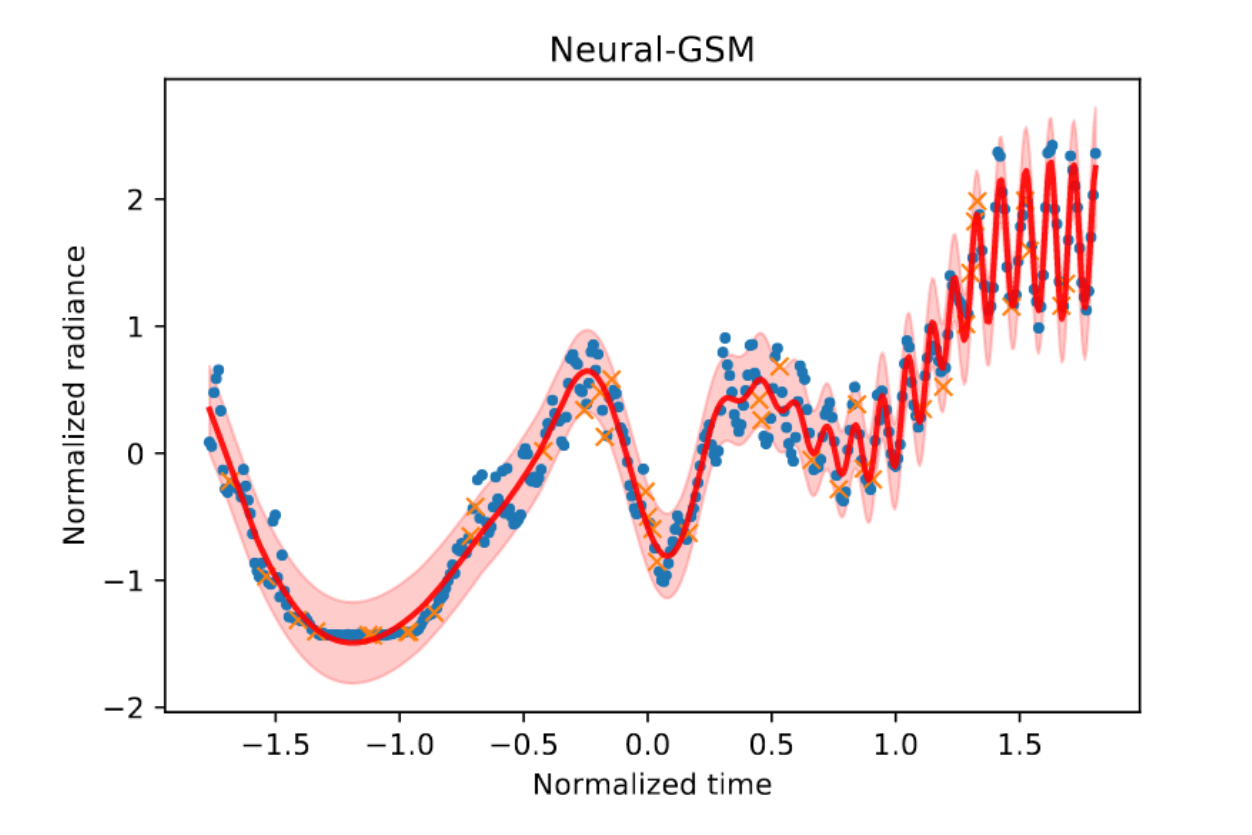
\includegraphics[width=.9\linewidth]{./niceplot.png}
\end{center}

Provides state-of-the-art performance on test data
\end{frame}

\begin{frame}[plain,label={sec:org2e5337a}]{My results}
\begin{center}
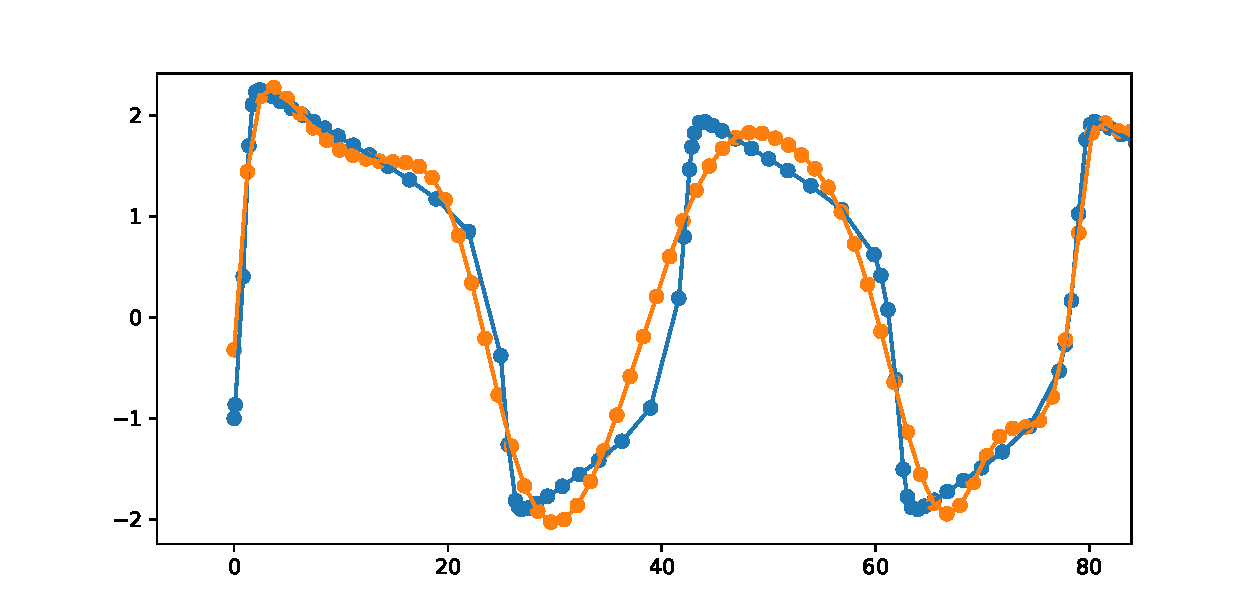
\includegraphics[width=\textwidth]{./neural_gsm.pdf}
\end{center}

It does look to have varying lengthscales, but it doesn't work well!
\end{frame}

\begin{frame}[label={sec:orgf7176fb}]{Possible issues}
\begin{itemize}
\item I don't trust the code
\begin{itemize}
\item Provided code relies on outdated, incompatible tensorflow, GPFlow versions; wouldn't run
\item I rewrote so it would run, but don't know tensorflow, GPFlow, so bad fit could be a code issue
\end{itemize}
\item Not enough data?
\item Bad training?
\begin{itemize}
\item I don't know anything about the tensorflow optimizers
\end{itemize}
\item Generally bad method?
\begin{itemize}
\item This was tested using algos from a preprint
\item A near-identical algo was published in a conference, might work better?
\end{itemize}
\end{itemize}
\end{frame}

\begin{frame}[label={sec:org03061d9}]{Other approaches}
Try other nonstationary kernels, or\ldots{}
\vfill
\begin{itemize}
\item Could use a good stationary kernel and hope its good enough
\item Real neurons have very short, fast spikes. Could use one kernel for the spikes, and another for the rest
\item GPFlow implements a switching kernel
\begin{itemize}
\item Develop some sort of algo to detect where to switch kernels
\item Fit a switching kernel, based around these changepoints
\end{itemize}
\item Could use hidden Markov chains for a piecewise model
\end{itemize}
\end{frame}

\begin{frame}[plain,label={sec:orgaa1f207}]{Other nonstationary kernels}
\begin{center}
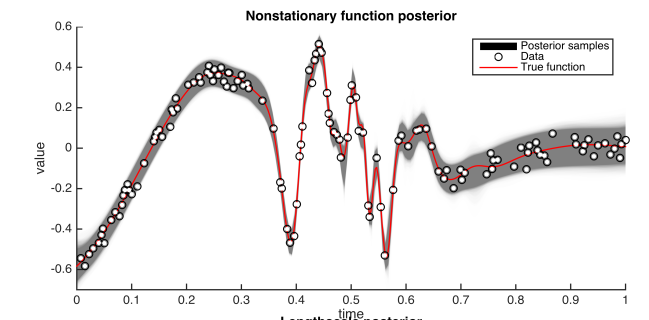
\includegraphics[width=.9\linewidth]{./nonstationary.png}
\end{center}

Source: Heinonen, Markus, et al. "Non-stationary gaussian process regression with hamiltonian monte carlo." Artificial Intelligence and Statistics. 2016.

\vfill

Similar idea to the method I already tried, but hopefully with more usable code.
\end{frame}

\begin{frame}[label={sec:orgde41d44}]{Hidden Markov chain model}
\begin{itemize}
\item Assume there's two dynamics, \(f_q(t)\) for quiescence, \(f_s(t)\) for spiking
\item Each dynamics are modelled as a random process
\item Hidden (latent) variable \(\theta\) dictates whether the neuron is spiking or quiescent
\item \(\theta\) follows a random process to initiate the transition from quiescence to spiking
\item Model:
\end{itemize}
\begin{equation}
f(t,\theta) = 
\begin{cases}
f_q(t) & \quad \text{if } \theta=0\\
f_s(t) & \quad \text{if } \theta=1
\end{cases}
\end{equation}
    \vfill 
Might be easy, might be hard
\end{frame}

\begin{frame}[plain,label={sec:org0fb446c}]{Good stationary kernel}
\begin{center}
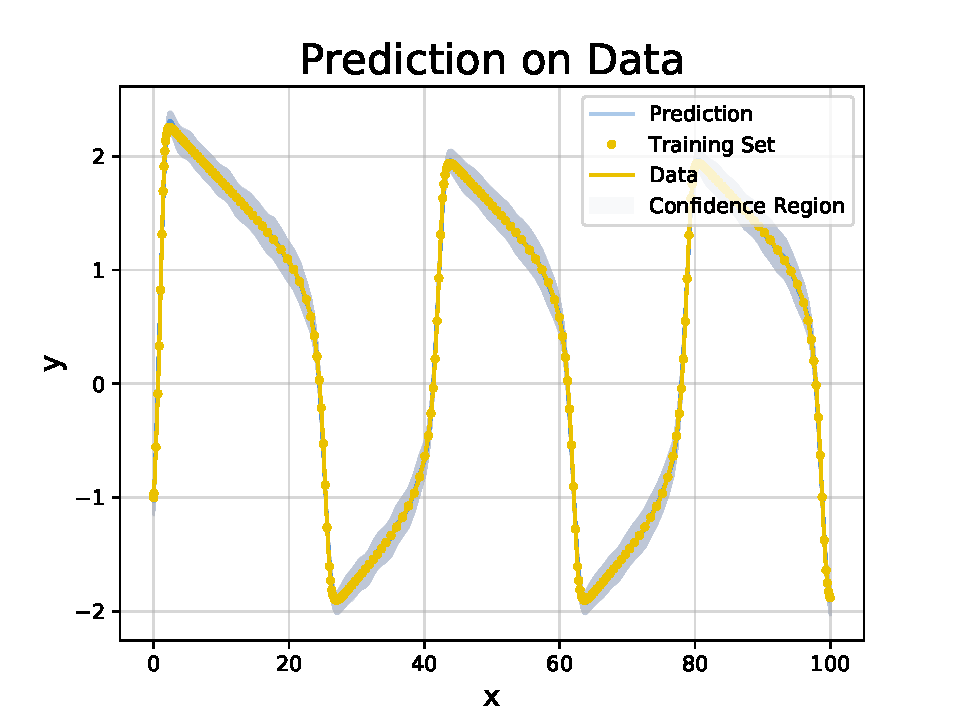
\includegraphics[width=.8\textwidth]{./fkl_1.pdf}
\end{center}

Uses the function-space distribution over kernels method; code adapted from

\url{https://github.com/wjmaddox/spectralgp}
\end{frame}

\begin{frame}[plain,label={sec:org5bc94a7}]{Good stationary kernel}
\begin{center}
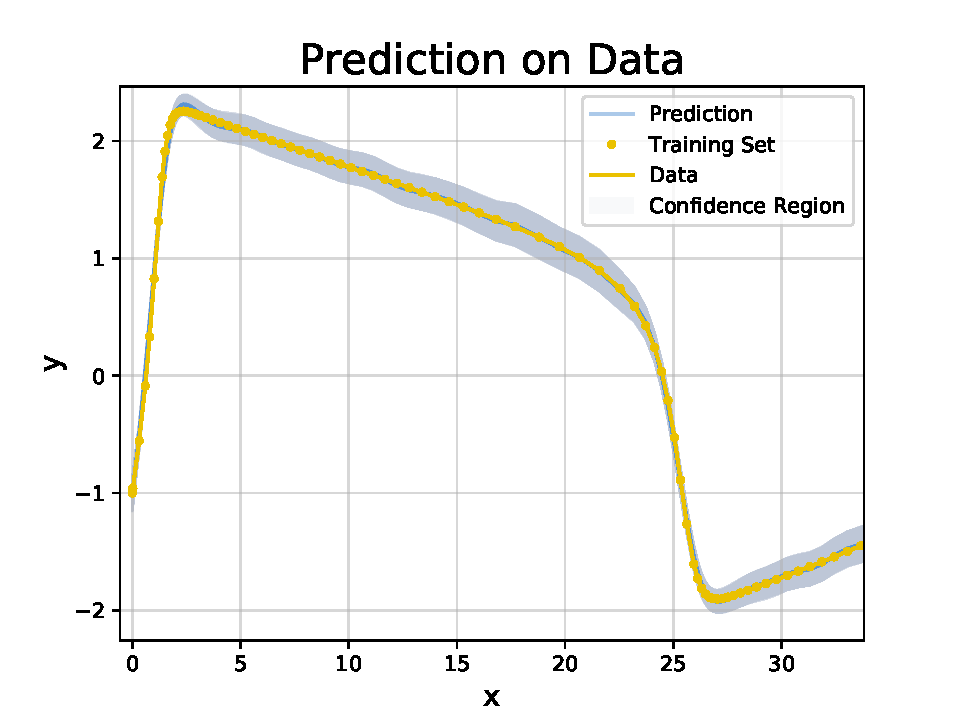
\includegraphics[width=.8\textwidth]{./fkl_2.pdf}
\end{center}

Uses the function-space distribution over kernels method; code adapted from

\url{https://github.com/wjmaddox/spectralgp}
\end{frame}

\begin{frame}[label={sec:org8dda83a}]{Good stationary kernel}
Caveat: 
\begin{itemize}
\item Fitzhugh-Nagumo is slower changing than real neuron data
\begin{itemize}
\item Real data would likely be strongly nonstationary, in which case this wouldn't work
\vfill
\end{itemize}
\item Good stationary kernels would be useful for a switching kernel, or a hidden Markov chain model
\begin{itemize}
\item Have a good stationary kernel for the active phase
\item Have a good stationary kernel for the quiescent phase
\item Switch between them at the appropriate points
\end{itemize}
\end{itemize}
\end{frame}

\begin{frame}[label={sec:orgc95310a}]{Good stationary kernel}
Note:
\begin{itemize}
\item The stationary method shown here is a spectral mixture kernel  -- SMK
\item The unsuccessful method was a generalised (nonstationary) spectral mixture kernel -- GSMK
\item A GSMK can model any SMK
\begin{itemize}
\item Anything an SMK can model, a GSMK can model equally well
\item Reverse is not true
\end{itemize}
\item Unsuccessful results are likely down to practice (coding issues), rather than theory (invalid kernel choice)
\end{itemize}
\end{frame}

\begin{frame}[label={sec:org8019c5b}]{Sidenote on GPFlow}
\begin{itemize}
\item Based on tensorflow
\begin{itemize}
\item Very fast, very powerful
\end{itemize}
\item Lots of the SOTA work uses GPFlow or GPyTorch
\item Might be worth learning how to use it
\begin{itemize}
\item Can implement and test more advanced kernels that way
\end{itemize}
\end{itemize}
\end{frame}

\section{Next steps}
\label{sec:org74577cc}
\begin{frame}[label={sec:orgb1a5ed2}]{Next steps}
\begin{itemize}
\item GPs are tricky on fast-changing data; I still think they'd be useful / worth the time and effort:
\begin{itemize}
\item Clean data source
\item Could allow CBC to be interfaced with existing continuation methods\ldots{}
\item \ldots{}or could be used to make a novel, application-specific / discretization-free continuation method

\vfill
\end{itemize}

\item More GPR testing
\begin{itemize}
\item Try other kernels (GPFlow periodic, Heinonen Hamiltonian Monte-Carlo, switching, \dots{})
\item Try to get GSM kernel to work?
\item Switching kernels?
\item Learn about Tensorflow and GPFlow?
\end{itemize}
\end{itemize}
\end{frame}
\end{document}
